
\section{复杂样板图样}

{\bfseries 知识目标}
\begin{itemize}
\item 掌握圆弧连接的绘制方法
\item 掌握图样的流程
\end{itemize}

{\bfseries 技能目标}
\begin{itemize}
\item 能够完成具有圆弧连接的复杂图样
\item 能够按照规范完成复杂图样抄绘
\end{itemize}

通过对本项目中\ref{sec:gongzhi}、\ref{sec:falan}和\ref{sec:yangban}的学习,我已经掌握了能够完成本项目刚开始所展示的图\ref{fig:xangmu1}那样复杂的图样。现在就让我们一步一步来完成这个复杂的图样,用激动人心的成果来结束该项目并检验的学习成果。
\subsection{设置绘图环境}
首先运用\ref{sec:gongzhi}中所学的方法将图形界限设置为$420\times 297$,接下来按照\ref{sec:falan}中所学的图层管理方法,新建绘制图\ref{fig:shangmu1}所需的中心线图层、细实线图层和粗实线图层,设置方法具体参见\ref{sec:gongzhi}和\ref{sec:falan}所述内容,此处不再赘述。
\subsection{绘制图框和标题栏}
根据图幅尺寸绘制图样的的边框:

\noindent
命令: RECTANG\\
指定第一个角点或 [倒角(C)/标高(E)/圆角(F)/厚度(T)/宽度(W)]: 0,0\\
指定另一个角点或 [面积(A)/尺寸(D)/旋转(R)]: 420,297\\
命令: RECTANG\\
指定第一个角点或 [倒角(C)/标高(E)/圆角(F)/厚度(T)/宽度(W)]: 25,10\\
指定另一个角点或 [面积(A)/尺寸(D)/旋转(R)]: 410,287\\

\indent
接下来根据图\ref{fig:biaotilan1}所示的尺寸绘制学生用标题栏。

\noindent
命令: line 指定第一点: 240,0\\
指定下一点或 [放弃(U)]:$ @40<90$\\
指定下一点或 [放弃(U)]:$ @180<0$\\
指定下一点或 [闭合(C)/放弃(U)]:\\
命令: OFFSET\\
当前设置: 删除源=否  图层=源  OFFSETGAPTYPE=0\\
指定偏移距离或 [通过(T)/删除(E)/图层(L)]$ <$通过$>$:  8\\
选择要偏移的对象,或 [退出(E)/放弃(U)]$ <$退出$>$:\\
指定要偏移的那一侧上的点,或 [退出(E)/多个(M)/放弃(U)]$ <$退出$>$:\\
选择要偏移的对象,或 [退出(E)/放弃(U)]$ <$退出$>$:\\
指定要偏移的那一侧上的点,或 [退出(E)/多个(M)/放弃(U)] $<$退出$>$:\\
选择要偏移的对象,或 [退出(E)/放弃(U)] $<$退出$>$:\\
指定要偏移的那一侧上的点,或 [退出(E)/多个(M)/放弃(U)] $<$退出$>$:\\
选择要偏移的对象,或 [退出(E)/放弃(U)] $<$退出$>$:\\
指定要偏移的那一侧上的点,或 [退出(E)/多个(M)/放弃(U)] $<$退出$>$:\\
选择要偏移的对象,或 [退出(E)/放弃(U)] $<$退出$>$:\\
命令: OFFSET\\
当前设置: 删除源=否  图层=源  OFFSETGAPTYPE=0\\
指定偏移距离或 [通过(T)/删除(E)/图层(L)] $<$8.0000$>$:  15\\
选择要偏移的对象,或 [退出(E)/放弃(U)] $<$退出$>$:\\
指定要偏移的那一侧上的点,或 [退出(E)/多个(M)/放弃(U)]$ <$退出$>$:\\
选择要偏移的对象,或 [退出(E)/放弃(U)] $<$退出$>$:\\
命令:  OFFSET\\
当前设置: 删除源=否  图层=源  OFFSETGAPTYPE=0\\
指定偏移距离或 [通过(T)/删除(E)/图层(L)]$ <$15.0000$>$:  30\\
选择要偏移的对象,或 [退出(E)/放弃(U)] $<$退出$>$:\\
指定要偏移的那一侧上的点,或 [退出(E)/多个(M)/放弃(U)]$ <$退出$>$:\\
选择要偏移的对象,或 [退出(E)/放弃(U)] $<$退出$>$:\\
命令:  OFFSET\\
当前设置: 删除源=否  图层=源  OFFSETGAPTYPE=0\\
指定偏移距离或 [通过(T)/删除(E)/图层(L)] $<$30.0000$>$:  15\\
选择要偏移的对象,或 [退出(E)/放弃(U)] $<$退出$>$:
指定要偏移的那一侧上的点,或 [退出(E)/多个(M)/放弃(U)]$ <$退出$>$:\\
选择要偏移的对象,或 [退出(E)/放弃(U)] $<$退出$>$:\\
命令:  OFFSET\\
当前设置: 删除源=否  图层=源  OFFSETGAPTYPE=0\\
指定偏移距离或 [通过(T)/删除(E)/图层(L)]$ <$15.0000$>$:  30\\
选择要偏移的对象,或 [退出(E)/放弃(U)] $<$退出$>$:\\
指定要偏移的那一侧上的点,或 [退出(E)/多个(M)/放弃(U)] $<$退出$>$:\\
选择要偏移的对象,或 [退出(E)/放弃(U)] $<$退出$>$:\\
命令:  OFFSET\\
当前设置: 删除源=否  图层=源  OFFSETGAPTYPE=0\\
指定偏移距离或 [通过(T)/删除(E)/图层(L)] $<$30.0000$>$:  45\\
选择要偏移的对象,或 [退出(E)/放弃(U)] $<$退出$>$:\\
指定要偏移的那一侧上的点,或 [退出(E)/多个(M)/放弃(U)]$ <$退出$>$:\\
选择要偏移的对象,或 [退出(E)/放弃(U)] $<$退出$>$:\\
命令:  OFFSET\\
当前设置: 删除源=否  图层=源  OFFSETGAPTYPE=0\\
指定偏移距离或 [通过(T)/删除(E)/图层(L)]$ <$45.0000$>$:  15\\
选择要偏移的对象,或 [退出(E)/放弃(U)] $<$退出$>$:\\
指定要偏移的那一侧上的点,或 [退出(E)/多个(M)/放弃(U)] $<$退出$>$:\\
选择要偏移的对象,或 [退出(E)/放弃(U)] $<$退出$>$:\\
命令: TRIM\\
当前设置:投影=UCS,边=无\\
选择剪切边...\\
选择对象或 $<$全部选择$>$:  找到 1 个\\
选择对象: 找到 1 个,总计 2 个\\
选择对象:\\
选择要修剪的对象,或按住 Shift 键选择要延伸的对象,或
[栏选(F)/窗交(C)/投影(P)/边(E)/删除(R)/放弃(U)]:\\
选择要修剪的对象,或按住 Shift 键选择要延伸的对象,或
[栏选(F)/窗交(C)/投影(P)/边(E)/删除(R)/放弃(U)]:\\
选择要修剪的对象,或按住 Shift 键选择要延伸的对象,或
[栏选(F)/窗交(C)/投影(P)/边(E)/删除(R)/放弃(U)]:\\
选择要修剪的对象,或按住 Shift 键选择要延伸的对象,或
[栏选(F)/窗交(C)/投影(P)/边(E)/删除(R)/放弃(U)]:\\
选择要修剪的对象,或按住 Shift 键选择要延伸的对象,或
[栏选(F)/窗交(C)/投影(P)/边(E)/删除(R)/放弃(U)]:\\
选择要修剪的对象,或按住 Shift 键选择要延伸的对象,或
[栏选(F)/窗交(C)/投影(P)/边(E)/删除(R)/放弃(U)]:\\
命令:  TRIM\\
当前设置:投影=UCS,边=无\\
选择剪切边...\\
选择对象或 $<$全部选择$>$:  找到 1 个\\
选择对象: 找到 1 个,总计 2 个\\
选择对象:\\
选择要修剪的对象,或按住 Shift 键选择要延伸的对象,或
[栏选(F)/窗交(C)/投影(P)/边(E)/删除(R)/放弃(U)]:\\
选择要修剪的对象,或按住 Shift 键选择要延伸的对象,或
[栏选(F)/窗交(C)/投影(P)/边(E)/删除(R)/放弃(U)]:\\
选择要修剪的对象,或按住 Shift 键选择要延伸的对象,或
[栏选(F)/窗交(C)/投影(P)/边(E)/删除(R)/放弃(U)]:\\
选择要修剪的对象,或按住 Shift 键选择要延伸的对象,或
[栏选(F)/窗交(C)/投影(P)/边(E)/删除(R)/放弃(U)]:\\
选择要修剪的对象,或按住 Shift 键选择要延伸的对象,或
[栏选(F)/窗交(C)/投影(P)/边(E)/删除(R)/放弃(U)]:\\

\indent
\subsection{绘制已经线段图形}

\noindent
命令: POINT\\
当前点模式:  PDMODE=0  PDSIZE=0.0000\\
指定点:\\
命令: XLINE \\
指定点或 [水平(H)/垂直(V)/角度(A)/二等分(B)/偏移(O)]: @109.5,90\\
指定通过点: @1$<$0\\
指定通过点: @1$<$90\\
指定通过点:\\
命令: CIRCLE \\
指定圆的圆心或 [三点(3P)/两点(2P)/切点、切点、半径(T)]: int 于\\
指定圆的半径或 [直径(D)]: 10\\
命令:  CIRCLE \\
指定圆的圆心或 [三点(3P)/两点(2P)/切点、切点、半径(T)]: int 于\\
指定圆的半径或 [直径(D)] $<$10.0000$>$: 18\\

命令: OFFSET\\
当前设置: 删除源=否  图层=源  OFFSETGAPTYPE=0\\
指定偏移距离或 [通过(T)/删除(E)/图层(L)] $<$通过$>$:  30\\
选择要偏移的对象,或 [退出(E)/放弃(U)] $<$退出$>$:\\
指定要偏移的那一侧上的点,或 [退出(E)/多个(M)/放弃(U)]$<$退出$>$:\\
选择要偏移的对象,或 [退出(E)/放弃(U)] $<$退出$>$:\\
命令:  OFFSET\\
当前设置: 删除源=否  图层=源  OFFSETGAPTYPE=0\\
指定偏移距离或 [通过(T)/删除(E)/图层(L)]$ <$30.0000$>$:  56\\
选择要偏移的对象,或 [退出(E)/放弃(U)] $<$退出$>$:\\
指定要偏移的那一侧上的点,或 [退出(E)/多个(M)/放弃(U)] $<$退出$>$:\\
选择要偏移的对象,或 [退出(E)/放弃(U)] $<$退出$>$:\\
命令: CIRCLE \\
指定圆的圆心或 [三点(3P)/两点(2P)/切点、切点、半径(T)]: int 于\\
指定圆的半径或 [直径(D)]$ <$20.0000$>$: 38\\
命令: offset\\
当前设置: 删除源=否  图层=源  OFFSETGAPTYPE=0\\
指定偏移距离或 [通过(T)/删除(E)/图层(L)] $<56.0000>$:  2\\
选择要偏移的对象,或 [退出(E)/放弃(U)]$ <$退出$>$:\\
指定要偏移的那一侧上的点,或 [退出(E)/多个(M)/放弃(U)]$<$退出$>$:\\
选择要偏移的对象,或 [退出(E)/放弃(U)] $<$退出$>$:\\
命令: TRIM\\
当前设置:投影=UCS,边=无\\
选择剪切边...\\
选择对象或 $<$全部选择$>$:  找到 1 个\\
选择对象:\\
选择要修剪的对象,或按住 Shift 键选择要延伸的对象,或
[栏选(F)/窗交(C)/投影(P)/边(E)/删除(R)/放弃(U)]:\\
选择要修剪的对象,或按住 Shift 键选择要延伸的对象,或
[栏选(F)/窗交(C)/投影(P)/边(E)/删除(R)/放弃(U)]:\\
选择要修剪的对象,或按住 Shift 键选择要延伸的对象,或
[栏选(F)/窗交(C)/投影(P)/边(E)/删除(R)/放弃(U)]:\\
选择要修剪的对象,或按住 Shift 键选择要延伸的对象,或
[栏选(F)/窗交(C)/投影(P)/边(E)/删除(R)/放弃(U)]:\\
选择要修剪的对象,或按住 Shift 键选择要延伸的对象,或
[栏选(F)/窗交(C)/投影(P)/边(E)/删除(R)/放弃(U)]:\\
命令: erase\\
选择对象: 找到 1 个\\
选择对象:\\

命令: OFFSET\\
当前设置: 删除源=否  图层=源  OFFSETGAPTYPE=0\\
指定偏移距离或 [通过(T)/删除(E)/图层(L)] $<56.0000>$:  203\\
选择要偏移的对象,或 [退出(E)/放弃(U)] $<$退出$>$:\\
指定要偏移的那一侧上的点,或 [退出(E)/多个(M)/放弃(U)]$ <$退出$>$:\\
选择要偏移的对象,或 [退出(E)/放弃(U)] $<$退出$>$:\\
命令:  OFFSET\\
当前设置: 删除源=否  图层=源  OFFSETGAPTYPE=0\\
指定偏移距离或 [通过(T)/删除(E)/图层(L)]$ <203.0000>$:  26\\
选择要偏移的对象,或 [退出(E)/放弃(U)] $<$退出$>$:\\
指定要偏移的那一侧上的点,或 [退出(E)/多个(M)/放弃(U)] $<$退出$>$:\\
选择要偏移的对象,或 [退出(E)/放弃(U)] $<$退出$>$:\\
命令: CIRCLE \\
指定圆的圆心或 [三点(3P)/两点(2P)/切点、切点、半径(T)]: int 于\\
指定圆的半径或 [直径(D)] $<38.0000>$: 12\\
命令:  CIRCLE \\
指定圆的圆心或 [三点(3P)/两点(2P)/切点、切点、半径(T)]: int 于\\
指定圆的半径或 [直径(D)] $<12.0000>$: 22\\
命令: offset\\
当前设置: 删除源=否  图层=源  OFFSETGAPTYPE=0\\
指定偏移距离或 [通过(T)/删除(E)/图层(L)] $<26.0000>$:  2\\
选择要偏移的对象,或 [退出(E)/放弃(U)]$ <$退出$>$:\\
指定要偏移的那一侧上的点,或 [退出(E)/多个(M)/放弃(U)]$<$退出$>$:\\
选择要偏移的对象,或 [退出(E)/放弃(U)] $<$退出$>$:\\
命令: TRIM\\
当前设置:投影=UCS,边=无\\
选择剪切边...\\
选择对象或 $<$全部选择$>$:  找到 1 个\\
选择对象:\\
选择要修剪的对象,或按住 Shift 键选择要延伸的对象,或
[栏选(F)/窗交(C)/投影(P)/边(E)/删除(R)/放弃(U)]:\\
选择要修剪的对象,或按住 Shift 键选择要延伸的对象,或
[栏选(F)/窗交(C)/投影(P)/边(E)/删除(R)/放弃(U)]:\\
选择要修剪的对象,或按住 Shift 键选择要延伸的对象,或
[栏选(F)/窗交(C)/投影(P)/边(E)/删除(R)/放弃(U)]:\\
选择要修剪的对象,或按住 Shift 键选择要延伸的对象,或
[栏选(F)/窗交(C)/投影(P)/边(E)/删除(R)/放弃(U)]:\\
选择要修剪的对象,或按住 Shift 键选择要延伸的对象,或
[栏选(F)/窗交(C)/投影(P)/边(E)/删除(R)/放弃(U)]:\\
命令: erase\\
选择对象: 找到 1 个\\
选择对象:\\

命令: OFFSET\\
当前设置: 删除源=否  图层=源  OFFSETGAPTYPE=0\\
指定偏移距离或 [通过(T)/删除(E)/图层(L)] $<26.0000>$:  45\\
选择要偏移的对象,或 [退出(E)/放弃(U)] $<$退出$>$:\\
指定要偏移的那一侧上的点,或 [退出(E)/多个(M)/放弃(U)] $<$退出$>$:\\
选择要偏移的对象,或 [退出(E)/放弃(U)] $<$退出$>$:\\
命令:  OFFSET\\
当前设置: 删除源=否  图层=源  OFFSETGAPTYPE=0\\
指定偏移距离或 [通过(T)/删除(E)/图层(L)]$ <45.0000>$:  38\\
选择要偏移的对象,或 [退出(E)/放弃(U)] $<$退出$>$:\\
指定要偏移的那一侧上的点,或 [退出(E)/多个(M)/放弃(U)]$ <$退出$>$:\\
选择要偏移的对象,或 [退出(E)/放弃(U)] $<$退出$>$:
命令: CIRCLE \\
指定圆的圆心或 [三点(3P)/两点(2P)/切点、切点、半径(T)]: int 于\\
指定圆的半径或 [直径(D)]$ <$22.0000$>$: 14\\
命令:  CIRCLE \\
指定圆的圆心或 [三点(3P)/两点(2P)/切点、切点、半径(T)]: int 于\\
指定圆的半径或 [直径(D)] $<14.0000>$: 5\\

命令: offset\\
当前设置: 删除源=否  图层=源  OFFSETGAPTYPE=0\\
指定偏移距离或 [通过(T)/删除(E)/图层(L)] $<38.0000>$:  52\\
选择要偏移的对象,或 [退出(E)/放弃(U)]$ <$退出$>$:\\
指定要偏移的那一侧上的点,或 [退出(E)/多个(M)/放弃(U)] $<$退出$>$:\\
选择要偏移的对象,或 [退出(E)/放弃(U)]$ <$退出$>$:\\
命令:  OFFSET\\
当前设置: 删除源=否  图层=源  OFFSETGAPTYPE=0\\
指定偏移距离或 [通过(T)/删除(E)/图层(L)] $<52.0000>$:  100\\
选择要偏移的对象,或 [退出(E)/放弃(U)] $<$退出$>$:\\
指定要偏移的那一侧上的点,或 [退出(E)/多个(M)/放弃(U)] $<$退出$>:$\\
选择要偏移的对象,或 [退出(E)/放弃(U)] $<$退出$>$:\\
命令: CIRCLE\\
指定圆的圆心或 [三点(3P)/两点(2P)/切点、切点、半径(T)]: int 于\\
指定圆的半径或 [直径(D)] <5.0000>: 5\\

命令: OFFSET\\
当前设置: 删除源=否  图层=源  OFFSETGAPTYPE=0\\
指定偏移距离或 [通过(T)/删除(E)/图层(L)] $<100.0000>$:  11\\
选择要偏移的对象,或 [退出(E)/放弃(U)]$ <$退出$>$:\\
指定要偏移的那一侧上的点,或 [退出(E)/多个(M)/放弃(U)]$ <$退出$>$:\\
选择要偏移的对象,或 [退出(E)/放弃(U)]$ <$退出$>$:\\
命令:  OFFSET\\
当前设置: 删除源=否  图层=源  OFFSETGAPTYPE=0\\
指定偏移距离或 [通过(T)/删除(E)/图层(L)] $<$11.0000$>$:  118\\
选择要偏移的对象,或 [退出(E)/放弃(U)] $<$退出$>$:\\
指定要偏移的那一侧上的点,或 [退出(E)/多个(M)/放弃(U)] $<$退出$>$:\\
选择要偏移的对象,或 [退出(E)/放弃(U)] $<$退出$>$:\\
命令: CIRCLE \\
指定圆的圆心或 [三点(3P)/两点(2P)/切点、切点、半径(T)]: int 于\\
指定圆的半径或 [直径(D)] $<5.0000>$: 5\\
命令: CIRCLE \\
指定圆的圆心或 [三点(3P)/两点(2P)/切点、切点、半径(T)]: int 于\\
指定圆的半径或 [直径(D)]$ <5.0000>$: 14\\

命令: OFFSET\\
当前设置: 删除源=否  图层=源  OFFSETGAPTYPE=0\\
指定偏移距离或 [通过(T)/删除(E)/图层(L)]$ <118.0000>$:  36\\
选择要偏移的对象,或 [退出(E)/放弃(U)]$ <$退出$>$:\\
指定要偏移的那一侧上的点,或 [退出(E)/多个(M)/放弃(U)]$ <$退出$>$:\\
选择要偏移的对象,或 [退出(E)/放弃(U)]$ <$退出$>$:\\
命令:  OFFSET\\
当前设置: 删除源=否  图层=源  OFFSETGAPTYPE=0\\
指定偏移距离或 [通过(T)/删除(E)/图层(L)] $<36.0000>$:  20\\
选择要偏移的对象,或 [退出(E)/放弃(U)] $<$退出$>$:\\
指定要偏移的那一侧上的点,或 [退出(E)/多个(M)/放弃(U)] $<$退出$>$:\\
选择要偏移的对象,或 [退出(E)/放弃(U)] $<$退出$>$:\\
命令: CIRCLE \\
指定圆的圆心或 [三点(3P)/两点(2P)/切点、切点、半径(T)]: int 于\\
指定圆的半径或 [直径(D)] $<$14.0000$>$: 14\\

命令:offset\\
当前设置: 删除源=否  图层=源  OFFSETGAPTYPE=0\\
指定偏移距离或 [通过(T)/删除(E)/图层(L)]$ <20.0000>$:  2\\
选择要偏移的对象,或 [退出(E)/放弃(U)] $<$退出$>$:\\
指定要偏移的那一侧上的点,或 [退出(E)/多个(M)/放弃(U)]$ <$退出$>$:\\
选择要偏移的对象,或 [退出(E)/放弃(U)]$ <$退出$>$:\\
命令: trim\\
当前设置:投影=UCS,边=无\\
选择剪切边...\\
选择对象或 $<$全部选择$>$:  找到 1 个\\
选择对象:\\
选择要修剪的对象,或按住 Shift 键选择要延伸的对象,或
[栏选(F)/窗交(C)/投影(P)/边(E)/删除(R)/放弃(U)]:\\
选择要修剪的对象,或按住 Shift 键选择要延伸的对象,或
[栏选(F)/窗交(C)/投影(P)/边(E)/删除(R)/放弃(U)]:\\
选择要修剪的对象,或按住 Shift 键选择要延伸的对象,或
[栏选(F)/窗交(C)/投影(P)/边(E)/删除(R)/放弃(U)]:\\
选择要修剪的对象,或按住 Shift 键选择要延伸的对象,或
[栏选(F)/窗交(C)/投影(P)/边(E)/删除(R)/放弃(U)]:\\
选择要修剪的对象,或按住 Shift 键选择要延伸的对象,或
[栏选(F)/窗交(C)/投影(P)/边(E)/删除(R)/放弃(U)]:\\
命令: erase\\
选择对象: 找到 1 个\\
选择对象:\\

命令:offset\\
当前设置: 删除源=否  图层=源  OFFSETGAPTYPE=0\\
指定偏移距离或 [通过(T)/删除(E)/图层(L)]$ <2.0000>$: \\
选择要偏移的对象,或 [退出(E)/放弃(U)] $<$退出$>$:\\
指定要偏移的那一侧上的点,或 [退出(E)/多个(M)/放弃(U)]$ <$退出$>$:\\
选择要偏移的对象,或 [退出(E)/放弃(U)]$ <$退出$>$:\\
命令: trim\\
当前设置:投影=UCS,边=无\\
选择剪切边...\\
选择对象或 $<$全部选择$>$:  找到 1 个\\
选择对象:\\
选择要修剪的对象,或按住 Shift 键选择要延伸的对象,或
[栏选(F)/窗交(C)/投影(P)/边(E)/删除(R)/放弃(U)]:\\
选择要修剪的对象,或按住 Shift 键选择要延伸的对象,或
[栏选(F)/窗交(C)/投影(P)/边(E)/删除(R)/放弃(U)]:\\
选择要修剪的对象,或按住 Shift 键选择要延伸的对象,或
[栏选(F)/窗交(C)/投影(P)/边(E)/删除(R)/放弃(U)]:\\
选择要修剪的对象,或按住 Shift 键选择要延伸的对象,或
[栏选(F)/窗交(C)/投影(P)/边(E)/删除(R)/放弃(U)]:\\
选择要修剪的对象,或按住 Shift 键选择要延伸的对象,或
[栏选(F)/窗交(C)/投影(P)/边(E)/删除(R)/放弃(U)]:\\
命令: erase\\
选择对象: 找到 1 个\\
选择对象:\\

命令:offset\\
当前设置: 删除源=否  图层=源  OFFSETGAPTYPE=0\\
指定偏移距离或 [通过(T)/删除(E)/图层(L)]$ <2.0000>$: \\
选择要偏移的对象,或 [退出(E)/放弃(U)] $<$退出$>$:\\
指定要偏移的那一侧上的点,或 [退出(E)/多个(M)/放弃(U)]$ <$退出$>$:\\
选择要偏移的对象,或 [退出(E)/放弃(U)]$ <$退出$>$:\\
命令: trim\\
当前设置:投影=UCS,边=无\\
选择剪切边...\\
选择对象或 $<$全部选择$>$:  找到 1 个\\
选择对象:\\
选择要修剪的对象,或按住 Shift 键选择要延伸的对象,或
[栏选(F)/窗交(C)/投影(P)/边(E)/删除(R)/放弃(U)]:\\
选择要修剪的对象,或按住 Shift 键选择要延伸的对象,或
[栏选(F)/窗交(C)/投影(P)/边(E)/删除(R)/放弃(U)]:\\
选择要修剪的对象,或按住 Shift 键选择要延伸的对象,或
[栏选(F)/窗交(C)/投影(P)/边(E)/删除(R)/放弃(U)]:\\
选择要修剪的对象,或按住 Shift 键选择要延伸的对象,或
[栏选(F)/窗交(C)/投影(P)/边(E)/删除(R)/放弃(U)]:\\
选择要修剪的对象,或按住 Shift 键选择要延伸的对象,或
[栏选(F)/窗交(C)/投影(P)/边(E)/删除(R)/放弃(U)]:\\
命令: erase\\
选择对象: 找到 1 个\\
选择对象:\\

命令:offset\\
当前设置: 删除源=否  图层=源  OFFSETGAPTYPE=0\\
指定偏移距离或 [通过(T)/删除(E)/图层(L)]$ <2.0000>$: \\
选择要偏移的对象,或 [退出(E)/放弃(U)] $<$退出$>$:\\
指定要偏移的那一侧上的点,或 [退出(E)/多个(M)/放弃(U)]$ <$退出$>$:\\
选择要偏移的对象,或 [退出(E)/放弃(U)]$ <$退出$>$:\\
命令: trim\\
当前设置:投影=UCS,边=无\\
选择剪切边...\\
选择对象或 $<$全部选择$>$:  找到 1 个\\
选择对象:\\
选择要修剪的对象,或按住 Shift 键选择要延伸的对象,或
[栏选(F)/窗交(C)/投影(P)/边(E)/删除(R)/放弃(U)]:\\
选择要修剪的对象,或按住 Shift 键选择要延伸的对象,或
[栏选(F)/窗交(C)/投影(P)/边(E)/删除(R)/放弃(U)]:\\
选择要修剪的对象,或按住 Shift 键选择要延伸的对象,或
[栏选(F)/窗交(C)/投影(P)/边(E)/删除(R)/放弃(U)]:\\
选择要修剪的对象,或按住 Shift 键选择要延伸的对象,或
[栏选(F)/窗交(C)/投影(P)/边(E)/删除(R)/放弃(U)]:\\
选择要修剪的对象,或按住 Shift 键选择要延伸的对象,或
[栏选(F)/窗交(C)/投影(P)/边(E)/删除(R)/放弃(U)]:\\
命令: erase\\
选择对象: 找到 1 个\\
选择对象:\\

\indent
完成上述绘图过程后,其结果如图\ref{fig:fuzatuyang1}所示。
\begin{figure}[htbp]
\centering
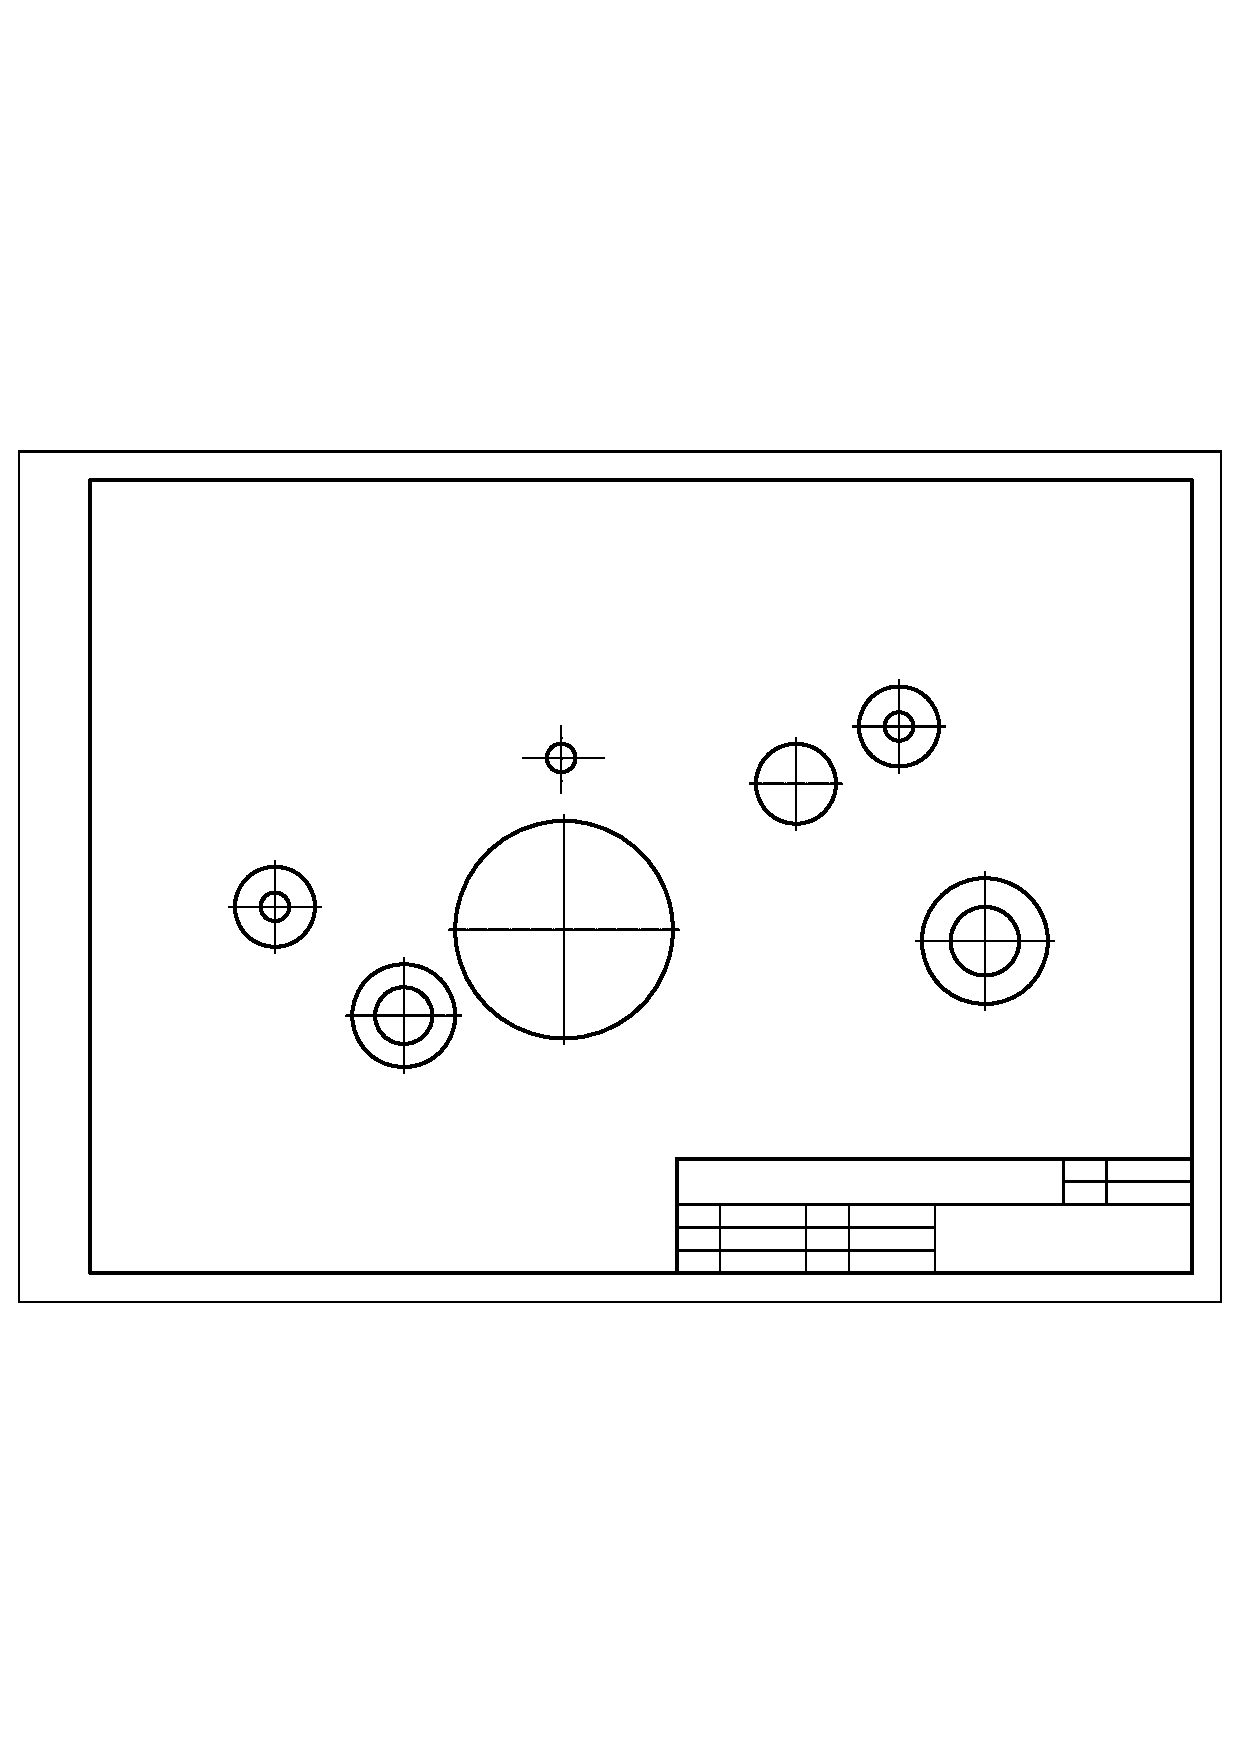
\includegraphics[scale=0.7]{fuzatuyang1.pdf}
\caption{复杂样板图样已知线段}\label{fig:fuzatuyang1}
\end{figure}
\subsection{绘制中间线段图形}
\noindent
命令: LINE\\
指定第一点: tan 到\\
指定下一点或 [放弃(U)]: $@50<0$\\
指定下一点或 [放弃(U)]:\\
命令: line 指定第一点: tan 到\\
指定下一点或 [放弃(U)]: $@-118<0$\\
指定下一点或 [放弃(U)]:\\
命令: LINE \\
指定第一点: tan 到\\
指定下一点或 [放弃(U)]: $@150<30$\\
指定下一点或 [放弃(U)]:\\
命令: LINE \\
指定第一点: tan 到\\
指定下一点或 [放弃(U)]:$ @30<90$\\
指定下一点或 [放弃(U)]:\\

\indent
\subsection{绘制连接线段图形}
\noindent
命令: fillet\\
当前设置: 模式 = 修剪,半径 = 0.0000\\
选择第一个对象或 [放弃(U)/多段线(P)/半径(R)/修剪(T)/多个(M)]: R \\
指定圆角半径$ <0.0000>$: 45
选择第一个对象或 [放弃(U)/多段线(P)/半径(R)/修剪(T)/多个(M)]:\\
选择第二个对象,或按住 Shift 键选择对象以应用角点或 [半径(R)]:\\
命令: fillet\\
当前设置: 模式 = 修剪,半径 = 45.0000\\
选择第一个对象或 [放弃(U)/多段线(P)/半径(R)/修剪(T)/多个(M)]: r\\
 指定圆角半径 $<45.0000>$: 20\\
选择第一个对象或 [放弃(U)/多段线(P)/半径(R)/修剪(T)/多个(M)]:\\
选择第二个对象,或按住 Shift 键选择对象以应用角点或 [半径(R)]:\\
命令: fillet\\
当前设置: 模式 = 修剪,半径 = 20.0000\\
选择第一个对象或 [放弃(U)/多段线(P)/半径(R)/修剪(T)/多个(M)]: r\\
指定圆角半径 $<20.0000>$: 10\\
选择第一个对象或 [放弃(U)/多段线(P)/半径(R)/修剪(T)/多个(M)]:\\
选择第二个对象,或按住 Shift 键选择对象以应用角点或 [半径(R)]:\\
命令: CIRCLE \\
指定圆的圆心或 [三点(3P)/两点(2P)/切点、切点、半径(T)]: t\\
指定对象与圆的第一个切点: tan 到\\
指定对象与圆的第二个切点:\\
指定圆的半径: 150\\
命令: CIRCLE \\
指定圆的圆心或 [三点(3P)/两点(2P)/切点、切点、半径(T)]: t\\
指定对象与圆的第一个切点:\\
指定对象与圆的第二个切点:\\
指定圆的半径 $<150.0000>$: 116\\
命令: trim\\
当前设置:投影=UCS,边=无\\
选择剪切边...\\
选择对象或$ <$全部选择$>$:  找到 1 个\\
选择对象: 找到 1 个,总计 2 个\\
选择对象: 找到 1 个,总计 3 个\\
选择对象: 找到 1 个,总计 4 个\\
选择对象: 找到 1 个,总计 5 个\\
选择对象: 找到 1 个,总计 6 个\\
选择对象:\\
选择要修剪的对象,或按住 Shift 键选择要延伸的对象,或
[栏选(F)/窗交(C)/投影(P)/边(E)/删除(R)/放弃(U)]:\\
选择要修剪的对象,或按住 Shift 键选择要延伸的对象,或
[栏选(F)/窗交(C)/投影(P)/边(E)/删除(R)/放弃(U)]:\\
选择要修剪的对象,或按住 Shift 键选择要延伸的对象,或
[栏选(F)/窗交(C)/投影(P)/边(E)/删除(R)/放弃(U)]:\\
选择要修剪的对象,或按住 Shift 键选择要延伸的对象,或
[栏选(F)/窗交(C)/投影(P)/边(E)/删除(R)/放弃(U)]:\\
命令: trim\\
当前设置:投影=UCS,边=无\\
选择剪切边...\\
选择对象或 $<$全部选择$>$:  找到 1 个\\
选择对象: 找到 1 个,总计 2 个\\
选择对象: 找到 1 个,总计 3 个\\
选择对象:\\
选择要修剪的对象,或按住 Shift 键选择要延伸的对象,或
[栏选(F)/窗交(C)/投影(P)/边(E)/删除(R)/放弃(U)]:\\
选择要修剪的对象,或按住 Shift 键选择要延伸的对象,或
[栏选(F)/窗交(C)/投影(P)/边(E)/删除(R)/放弃(U)]:\\
选择要修剪的对象,或按住 Shift 键选择要延伸的对象,或
[栏选(F)/窗交(C)/投影(P)/边(E)/删除(R)/放弃(U)]:\\
命令: trim\\
当前设置:投影=UCS,边=无\\
选择剪切边...\\
选择对象或$ <$全部选择$>$:  找到 1 个\\
选择对象: 找到 1 个,总计 2 个\\
选择对象:\\
选择要修剪的对象,或按住 Shift 键选择要延伸的对象,或
[栏选(F)/窗交(C)/投影(P)/边(E)/删除(R)/放弃(U)]:\\
选择要修剪的对象,或按住 Shift 键选择要延伸的对象,或
[栏选(F)/窗交(C)/投影(P)/边(E)/删除(R)/放弃(U)]:\\

\indent
完成所有的绘图过程后,其结果如\ref{fig:fuzatuyang2}所示。
\begin{figure}[htbp]
\centering
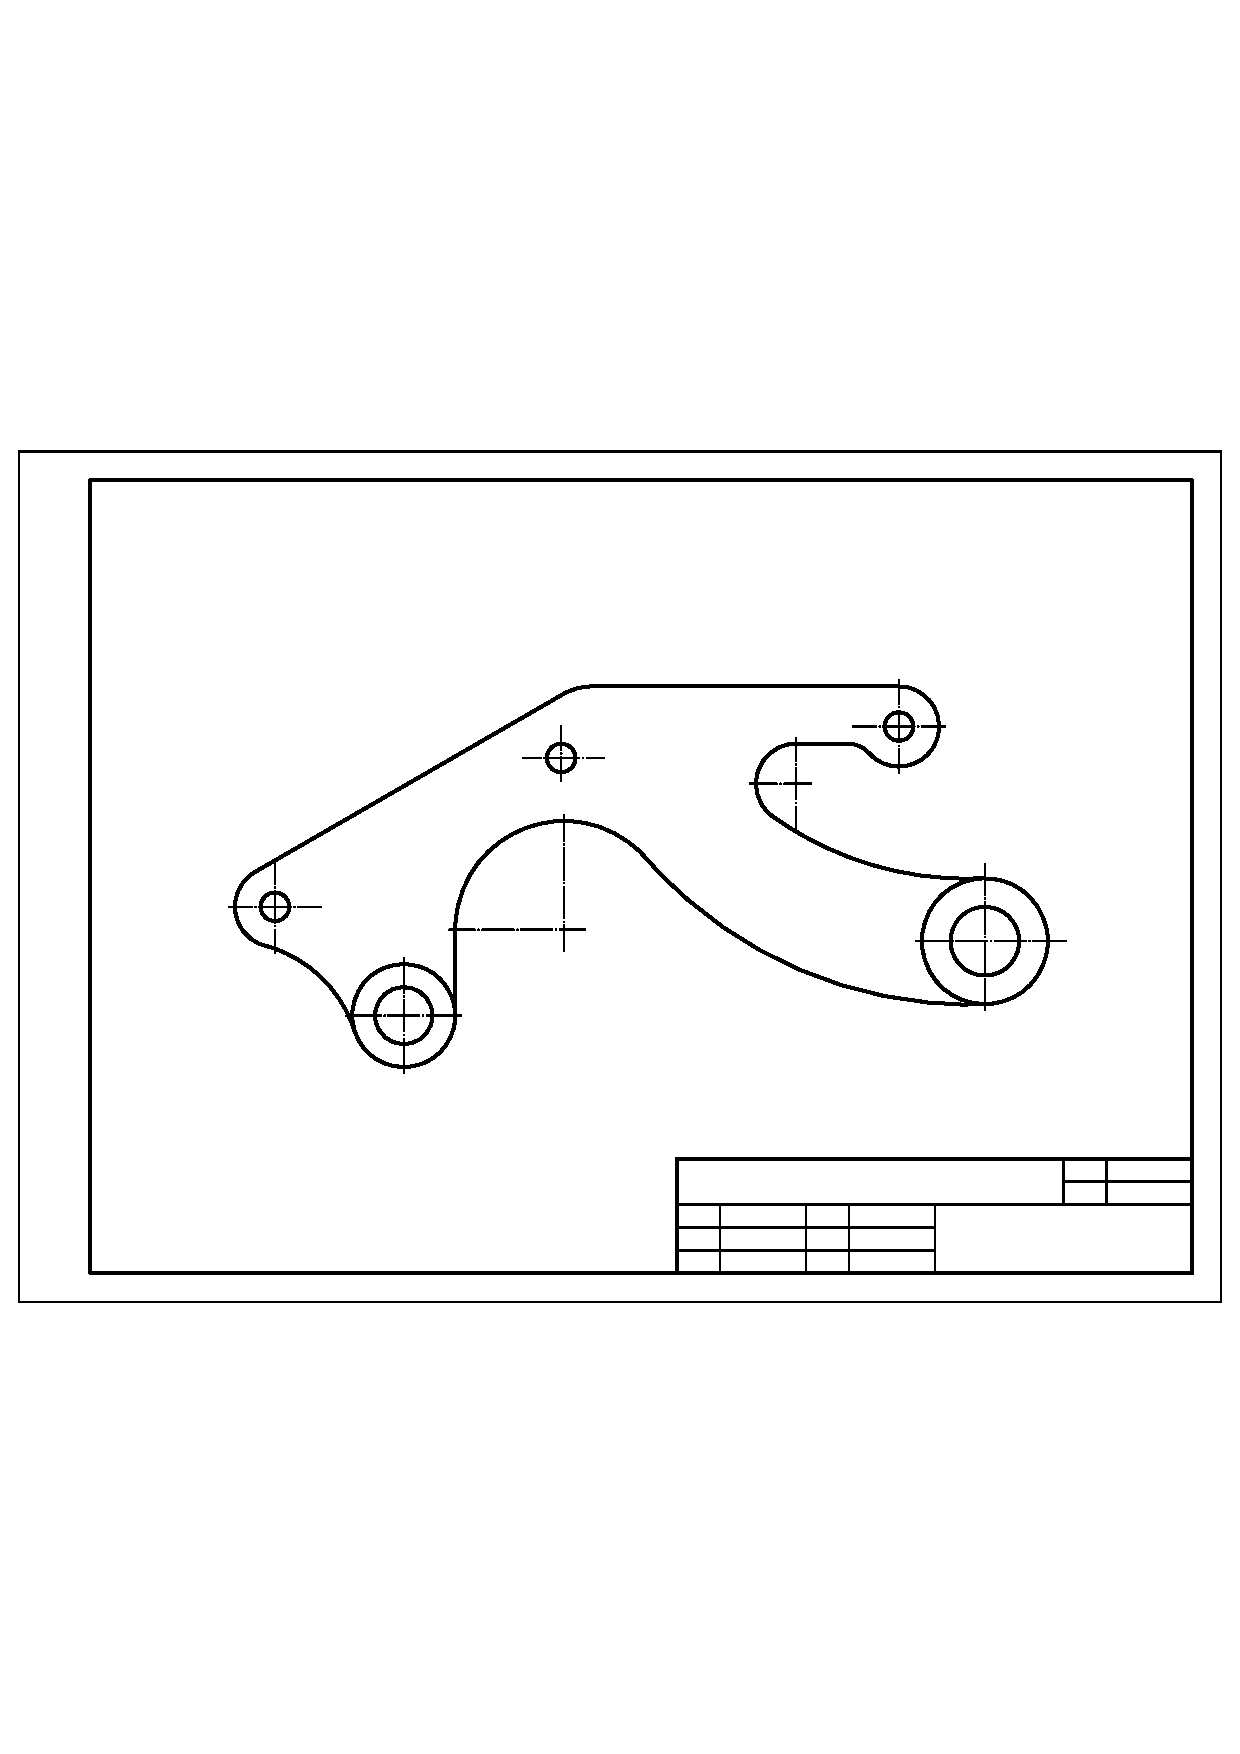
\includegraphics[scale=0.7]{fuzatuyang2.pdf}
\caption{复杂样板图样结果}\label{fig:fuzatuyang2}
\end{figure}
\endinput
